\subsection{\color{ForestGreen}Regular Expressions}
\subsubsection{Definitions}
\begin{itemize}
    \item Kleene closure: $L(E^*) = (L(E))^*$
\end{itemize}
\subsubsection{$\mathbf{Regex \implies \epsilon-NFA}$}
\begin{Figure}
    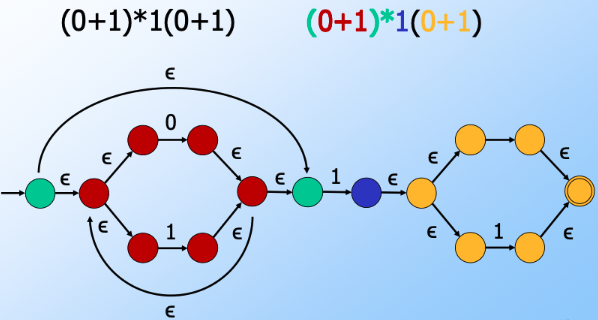
\includegraphics[width=0.7\linewidth]{figures/RE-NFA.png}
\end{Figure}
\subsubsection{$\mathbf{DFA \implies Regex}$}
\textbf{K-path induction}: $R_{ij}^ k = R_{ij}^{k-1} + R_{ik}^{k-1}(R_{kk}^{k-1})^* R_{kj} ^{k-1} $, where $R^k_{ij}$ is the Regex for the set of labels of k-paths from state $i$ to state $j.$
the final step of the k-path algorithm is to do the addition of all $R_{ij}^n$ where $n$ is the number of states, $i$ is the start state, $j$ are the accept states
